% 机器人系统设计大作业
% 题目：基于深度强化学习的H1人形机器人行走控制系统设计
% 编译：xelatex report.tex（需要中文支持）

\documentclass[12pt, a4paper]{article}

% ==================== 宏包 ====================
\usepackage{ctex}                     % 中文支持
\usepackage{geometry}
\geometry{left=2.5cm, right=2.5cm, top=3cm, bottom=3cm}
\usepackage{amsmath, amssymb}
\usepackage{graphicx}
\usepackage{booktabs}                 % 三线表
\usepackage{array}
\usepackage{multirow}
\usepackage{hyperref}
\usepackage{caption}
\usepackage{subcaption}
\usepackage{listings}                 % 代码块
\usepackage{xcolor}
\usepackage{setspace}
\usepackage{enumitem}
\usepackage{float}

% ==================== 代码样式 ====================
\lstset{
    basicstyle=\small\ttfamily,
    keywordstyle=\color{blue},
    commentstyle=\color{gray},
    stringstyle=\color{red},
    breaklines=true,
    frame=single,
    numbers=left,
    numberstyle=\tiny,
    xleftmargin=2em,
}

% ==================== 页眉页脚 ====================
\usepackage{fancyhdr}
\pagestyle{fancy}
\fancyhf{}
\lhead{机器人系统设计课程大作业}
\rhead{H1人形机器人行走控制系统}
\cfoot{\thepage}

% ==================== 标题信息 ====================
\title{
    \vspace{2cm}
    \textbf{\Large 基于深度强化学习的H1人形机器人\\行走控制系统设计}\\[1cm]
    \large 机器人系统设计课程大作业
    \vspace{1cm}
}
\author{
    姓名：\underline{\hspace{4cm}} \\[0.5em]
    学号：\underline{\hspace{4cm}} \\[0.5em]
    专业：\underline{\hspace{4cm}}
}
\date{\today}

% ==================== 正文 ====================
\begin{document}

\maketitle
\thispagestyle{empty}
\newpage

\tableofcontents
\newpage

% --------------------------------------------------
\section{设计目的}
% --------------------------------------------------

人形机器人的运动控制是机器人系统设计中最具挑战性的问题之一。
与传统工业机器人不同，人形机器人需要在非结构化环境中实时维持动态平衡，
对控制系统的实时性、鲁棒性和泛化能力提出了极高要求。

本课题以宇树（Unitree）H1人形机器人为平台，目标是：

\begin{enumerate}[label=(\arabic*)]
    \item 在物理仿真环境中，通过深度强化学习（Deep RL）训练一套可行走的控制策略；
    \item 搭建基于ROS2话题通信（\texttt{/imu} $\to$ \texttt{/cmd\_vel}）的闭环控制系统，
          使机器人能够依据预设的指令路径（直行、转弯、停止等分段指令序列）
          实时纠正航向偏差，完成指令路径的行走任务；
    \item 以\textbf{关节加速度惩罚系数}（$c_\text{dof\_acc}$）为消融变量，设计三组对照实验，
          定量分析其对动作平滑性、步态质量和速度跟踪精度的影响；
    \item 为后续在ROS2框架下部署到真实H1机器人提供基线模型与参数选取依据。
\end{enumerate}

% 关联课程内容的说明
本设计涵盖课程中的以下核心内容：
机器人系统架构设计、关节驱动需求分析、传感器与观测空间建模、控制算法设计与验证流程。


% --------------------------------------------------
\section{需求分析}
% --------------------------------------------------

\subsection{H1平台硬件参数}

Unitree H1是一款全尺寸人形机器人，关键参数如表~\ref{tab:h1_spec}所示。

\begin{table}[H]
\centering
\caption{Unitree H1关键硬件参数}
\label{tab:h1_spec}
\begin{tabular}{lll}
\toprule
参数 & 数值 & 说明 \\
\midrule
整机质量 & 47 kg & 含电池 \\
身高 & 1.8 m & — \\
控制自由度（DOF） & 10 & 仅下肢（髋×3+膝×1+踝×1，双侧） \\
关节控制频率 & 50 Hz & 上位机控制周期 20 ms \\
髋关节峰值力矩 & 200 Nm & — \\
膝关节峰值力矩 & 300 Nm & — \\
踝关节峰值力矩 & 45 Nm & — \\
传动方案 & PMSM + 行星减速器 & 力矩控制模式 \\
\bottomrule
\end{tabular}
\end{table}

\subsection{控制系统需求}

结合H1的硬件参数与实机部署目标，控制策略需满足以下需求：

\begin{enumerate}[label=(\arabic*)]
    \item \textbf{速度跟踪能力。} 策略须在 $v_x, v_y \in [-1.0, 1.0]$\,m/s 的线速度指令
          （含偏航角速度指令）下保持稳定行走，并准确跟踪指令方向与速度。
    \item \textbf{动作平滑性。} 相邻控制帧的关节力矩变化率须在安全范围内，
          以保护减速器齿轮和轴承，避免冲击载荷损伤传动部件。
    \item \textbf{躯干稳定性。} 行走过程中躯干俯仰/横滚角速度须被抑制，
          以维持传感器（IMU）的测量精度并避免摔倒。
    \item \textbf{计算实时性。} 策略推理须在20\,ms以内完成，满足50\,Hz实时控制要求。
\end{enumerate}

\subsection{关节加速度惩罚的工程动机}

在强化学习奖励函数中，关节加速度惩罚项定义为：

\begin{equation}
    r_\text{dof\_acc} = c_\text{dof\_acc} \cdot \sum_{i=1}^{N_\text{dof}} \ddot{q}_i^2
    \label{eq:dof_acc}
\end{equation}

其中 $c_\text{dof\_acc} < 0$ 为惩罚系数，$\ddot{q}_i$ 为第 $i$ 个关节的角加速度。

该惩罚项的工程背景源于传动系统的冲击载荷问题。
以H1膝关节为例（PMSM + 行星减速器，减速比约 $N = 20:1$），
关节侧角加速度 $\ddot{q}_\text{joint}$ 折算到电机侧为 $\ddot{q}_\text{motor} = N \cdot \ddot{q}_\text{joint}$，
电机转子的动态力矩为：

\begin{equation}
    \tau_\text{inertia} = J_\text{motor} \cdot \ddot{q}_\text{motor}
    = J_\text{motor} \cdot N \cdot \ddot{q}_\text{joint}
    \label{eq:inertia_torque}
\end{equation}

过大的关节加速度会导致电机电流尖峰，加速减速器磨损，
甚至在高减速比传动中产生超过额定值的冲击力矩。
因此，$c_\text{dof\_acc}$ 的合理选取是控制策略与机械系统协同设计的关键参数。


% --------------------------------------------------
\section{技术方案}
% --------------------------------------------------

\subsection{整体系统架构}

本设计采用"仿真训练 + 策略部署"的两阶段架构，如图~\ref{fig:architecture}所示。

% TODO：插入系统框图（可用tikz绘制或截图替代）
\begin{figure}[H]
\centering
\includegraphics[width=0.95\textwidth]{figs/architecture.png}
\caption{H1行走控制系统整体架构}
\label{fig:architecture}
\end{figure}

\begin{itemize}
    \item \textbf{仿真平台：} Genesis 1.0.0，CUDA后端并行仿真；
    \item \textbf{训练算法：} PPO（Proximal Policy Optimization），复刻rsl\_rl实现；
    \item \textbf{策略网络：} LSTM（hidden=64）+ MLP（[32]，ELU激活）；
    \item \textbf{并行环境数：} 8192个；
    \item \textbf{控制频率：} 50\,Hz；
    \item \textbf{ROS2集成：} 在仿真环境中通过 \texttt{/imu} $\to$ \texttt{/cmd\_vel}
          话题通信构建闭环路径跟踪验证（本设计未迁移至实机，实机部署留作后续工作）。
\end{itemize}

\subsection{观测空间设计}

策略的输入观测向量共41维，具体构成如表~\ref{tab:obs}所示。

\begin{table}[H]
\centering
\caption{观测空间构成（41维）}
\label{tab:obs}
\begin{tabular}{llr}
\toprule
类别 & 内容 & 维度 \\
\midrule
IMU & 躯干角速度（roll/pitch/yaw rate） & 3 \\
IMU & 重力方向在机体系的投影 & 3 \\
指令 & 线速度指令 $(v_x^*, v_y^*)$，偏航角速度指令 $\omega_z^*$ & 3 \\
关节状态 & 关节角度偏差 $q - q_\text{default}$ & 10 \\
关节状态 & 关节角速度 $\dot{q}$ & 10 \\
历史动作 & 上一步输出动作 $a_{t-1}$ & 10 \\
相位时钟 & $[\sin\phi, \cos\phi]$（双腿相位） & 2 \\
\midrule
\multicolumn{2}{l}{Critic额外观测（特权信息）} & +3 \\
\multicolumn{2}{l}{躯干线速度（仅训练时Critic使用）} & \\
\midrule
总计（Actor） & & 41 \\
总计（Critic） & & 44 \\
\bottomrule
\end{tabular}
\end{table}

\subsection{奖励函数设计}

奖励函数共包含15项，分为正向奖励（鼓励行为）和负向惩罚（抑制行为）两类，
整体结构参考了 Unitree \texttt{H1RoughCfg}（速度跟踪、姿态稳定、动作平滑、
步态时序等分项），并在此基础上对 \texttt{tracking\_lin\_vel}、\texttt{ang\_vel\_xy}、
\texttt{action\_rate}、\texttt{feet\_swing\_height}、\texttt{contact\_no\_vel}
以及作为消融变量的 \texttt{dof\_acc} 进行了调参；各分项的具体系数设置、
与参考实现的差异及设计意图见附录表~\ref{tab:reward}。

\subsection{消融实验设计}

本设计以关节加速度惩罚系数 $c_\text{dof\_acc}$ 为消融变量，设计三组实验，
其余所有超参数保持一致，如表~\ref{tab:ablation}所示。

\begin{table}[H]
\centering
\caption{消融实验分组设置}
\label{tab:ablation}
\begin{tabular}{llll}
\toprule
组别 & 模型名称 & $c_\text{dof\_acc}$ & 相对默认值倍率 \\
\midrule
基准组 & v4\_r48s & $-1 \times 10^{-6}$ & 4× \\
对比组1 & v4\_r48s\_acc5x & $-5 \times 10^{-6}$ & 20× \\
对比组2 & v4\_r48s\_acc10x & $-1 \times 10^{-5}$ & 40× \\
\bottomrule
\end{tabular}
\end{table}

三组实验均训练 $10000$ 个更新步（update），每步 rollout 长度为48，
并行环境数8192，对应约 $10000 \times 48 \times 8192 \approx 3.9 \times 10^9$ 个环境步。

\subsection{PPO算法关键参数}

\begin{table}[H]
\centering
\caption{PPO超参数设置}
\label{tab:ppo}
\begin{tabular}{lll}
\toprule
参数 & 数值 & 说明 \\
\midrule
学习率 & $10^{-3}$，自适应 $[10^{-5}, 10^{-2}]$ & KL散度目标0.01 \\
clip参数 & 0.2 & PPO裁剪范围 \\
熵系数 & 0.003 & 鼓励探索 \\
价值函数系数 & 1.0 & — \\
GAE参数 & $\gamma=0.99$，$\lambda=0.95$ & — \\
每轮epoch & 5 & — \\
mini-batch数 & 4 & — \\
梯度裁剪 & 1.0 & — \\
\bottomrule
\end{tabular}
\end{table}


% --------------------------------------------------
\section{测试结果}
% --------------------------------------------------

\subsection{训练收敛分析}

三组模型训练全程的奖励与价值损失曲线见附录图~\ref{fig:training_curve}（直接由
\texttt{train\_v4\_r48s*.log} 中每 10 个 update 记录一次的 \texttt{rew}/\texttt{vloss}
解析得到，细线为原始值、粗线为滑动平均）。从中可以观察到：

\begin{itemize}
    \item 三组模型的奖励曲线均在约 2000\,$\sim$\,3000 个 update 后进入收敛
          平台期，此后仅在小范围内波动；其中 acc10x 进入平台期的时间点明显
          更靠后，收敛速度慢于另外两组；
    \item 取末段（最后 50 个 update）奖励均值作为收敛水平：v4\_r48s
          $\approx 0.035$、acc5x $\approx 0.030$、acc10x $\approx 0.027$——
          acc10x 比基准组低约 $22\%$，与其在表~\ref{tab:eval_breakdown}中总奖励偏低的结果一致；由于acc5x和acc10x都对参数$c_\text{dof\_acc}$进行了不同程度的惩罚，因此最后的结果完全是在考虑范围之内。
    \item 三组的价值损失曲线均存在周期性抖动（约每 $120\sim130$ 个 update
          一次），属于 LSTM 策略梯度训练中的已知现象，不影响最终性能。
\end{itemize}

\subsection{奖励分项定量对比}

使用 \texttt{eval\_breakdown.py} 对三组模型（各取best checkpoint）进行
多速度（$0.3$\,m/s、$0.6$\,m/s、$0.9$\,m/s）评估，
核心分项结果汇总于表~\ref{tab:eval_breakdown}。

\begin{table}[H]
\centering
\caption{三组模型奖励分项对比（均值，$\pm$标准差）}
\label{tab:eval_breakdown}
\begin{tabular}{lrrr}
\toprule
奖励分项 & v4\_r48s & v4\_r48s\_acc5x & v4\_r48s\_acc10x \\
\midrule
tracking\_lin\_vel & $0.640\pm0.316$ & $0.680\pm0.280$ & $0.654\pm0.306$ \\
dof\_acc（×$10^{-3}$） & $51.26\pm20.52$ & $23.03\pm15.65$ & $27.40\pm12.56$ \\
action\_rate & $1.617\pm0.499$ & $1.510\pm0.304$ & $1.576\pm0.296$ \\
ang\_vel\_xy & $0.707\pm0.883$ & $0.445\pm0.743$ & $0.908\pm1.177$ \\
feet\_swing\_height（×$10^{3}$） & $0.754\pm0.932$ & $0.289\pm0.656$ & $0.946\pm1.979$ \\
contact\_no\_vel & $0.0842\pm0.110$ & $0.0711\pm0.137$ & $0.0901\pm0.130$ \\
\midrule
总奖励 & $0.0240\pm0.0090$ & $0.0265\pm0.0079$ & $0.0238\pm0.0088$ \\
\bottomrule
\end{tabular}
\end{table}

\noindent\footnotesize 注：表中各分项均为 \texttt{env.py} 的
\texttt{\_compute\_rewards} 计算得到的\textbf{原始（未加权）}奖励值 $r_k$，
实际计入总奖励的贡献为 $c_k \Delta t\, r_k$（系数 $c_k$ 见附录表~\ref{tab:reward}，
控制步长 $\Delta t = 0.02$\,s）。各分项的计算公式与量纲说明见
附录"奖励分项与平滑性指标的计算公式及量纲"。\par\normalsize

\subsection{步态质量与可视化}

通过 \texttt{play.py} 渲染三组模型的行走视频（\texttt{play\_best.mp4}，命令速度 $v_x = 0.5$\,m/s），并从中各截取 $t = 0\sim1.0$\,s（覆盖两个以上完整步态周期，步态周期约 $0.8$\,s）范围内的连续帧，以 $0.1$\,s 为间隔等间隔抽取 11 帧，按方案横向排布、纵向对比，如图~\ref{fig:gait}所示。

定性观察（结合图~\ref{fig:gait}与表~\ref{tab:eval_breakdown}中的 \texttt{feet\_swing\_height}、\texttt{contact\_no\_vel} 指标）：
\begin{itemize}
    \item v4\_r48s：摆动腿抬升幅度在三者中最不明显，落地点与支撑腿距离较近、步幅偏小，整体呈现出一定的“小碎步”特征，与其 \texttt{feet\_swing\_height} 均值（$1.04\times10^{-3}$）和 \texttt{contact\_no\_vel} 均值（$0.104$）处于三者中间水平相符；
    \item v4\_r48s\_acc5x：抬腿高度与步幅在三者中最小，迈步动作也最为紧凑、细碎，对应其 \texttt{feet\_swing\_height} 均值最低（$0.74\times10^{-3}$），意味着该方案在抑制关节加速度的同时进一步压低了摆动腿轨迹，"小碎步"现象相对最明显；
    \item v4\_r48s\_acc10x：抬腿高度和迈步幅度在三者中最大，步态周期内大腿摆动更充分、姿态更接近正常行走，但同时上半身摇摆幅度也更大，与其 \texttt{feet\_swing\_height}（$1.44\times10^{-3}$）和 \texttt{contact\_no\_vel}（$0.158$）均为三者最高、\texttt{ang\_vel\_xy}（$1.495$）显著偏大相印证——抬腿更高、落地拖滑更多、姿态稳定性也相应下降。
\end{itemize}

\begin{figure}[H]
\centering
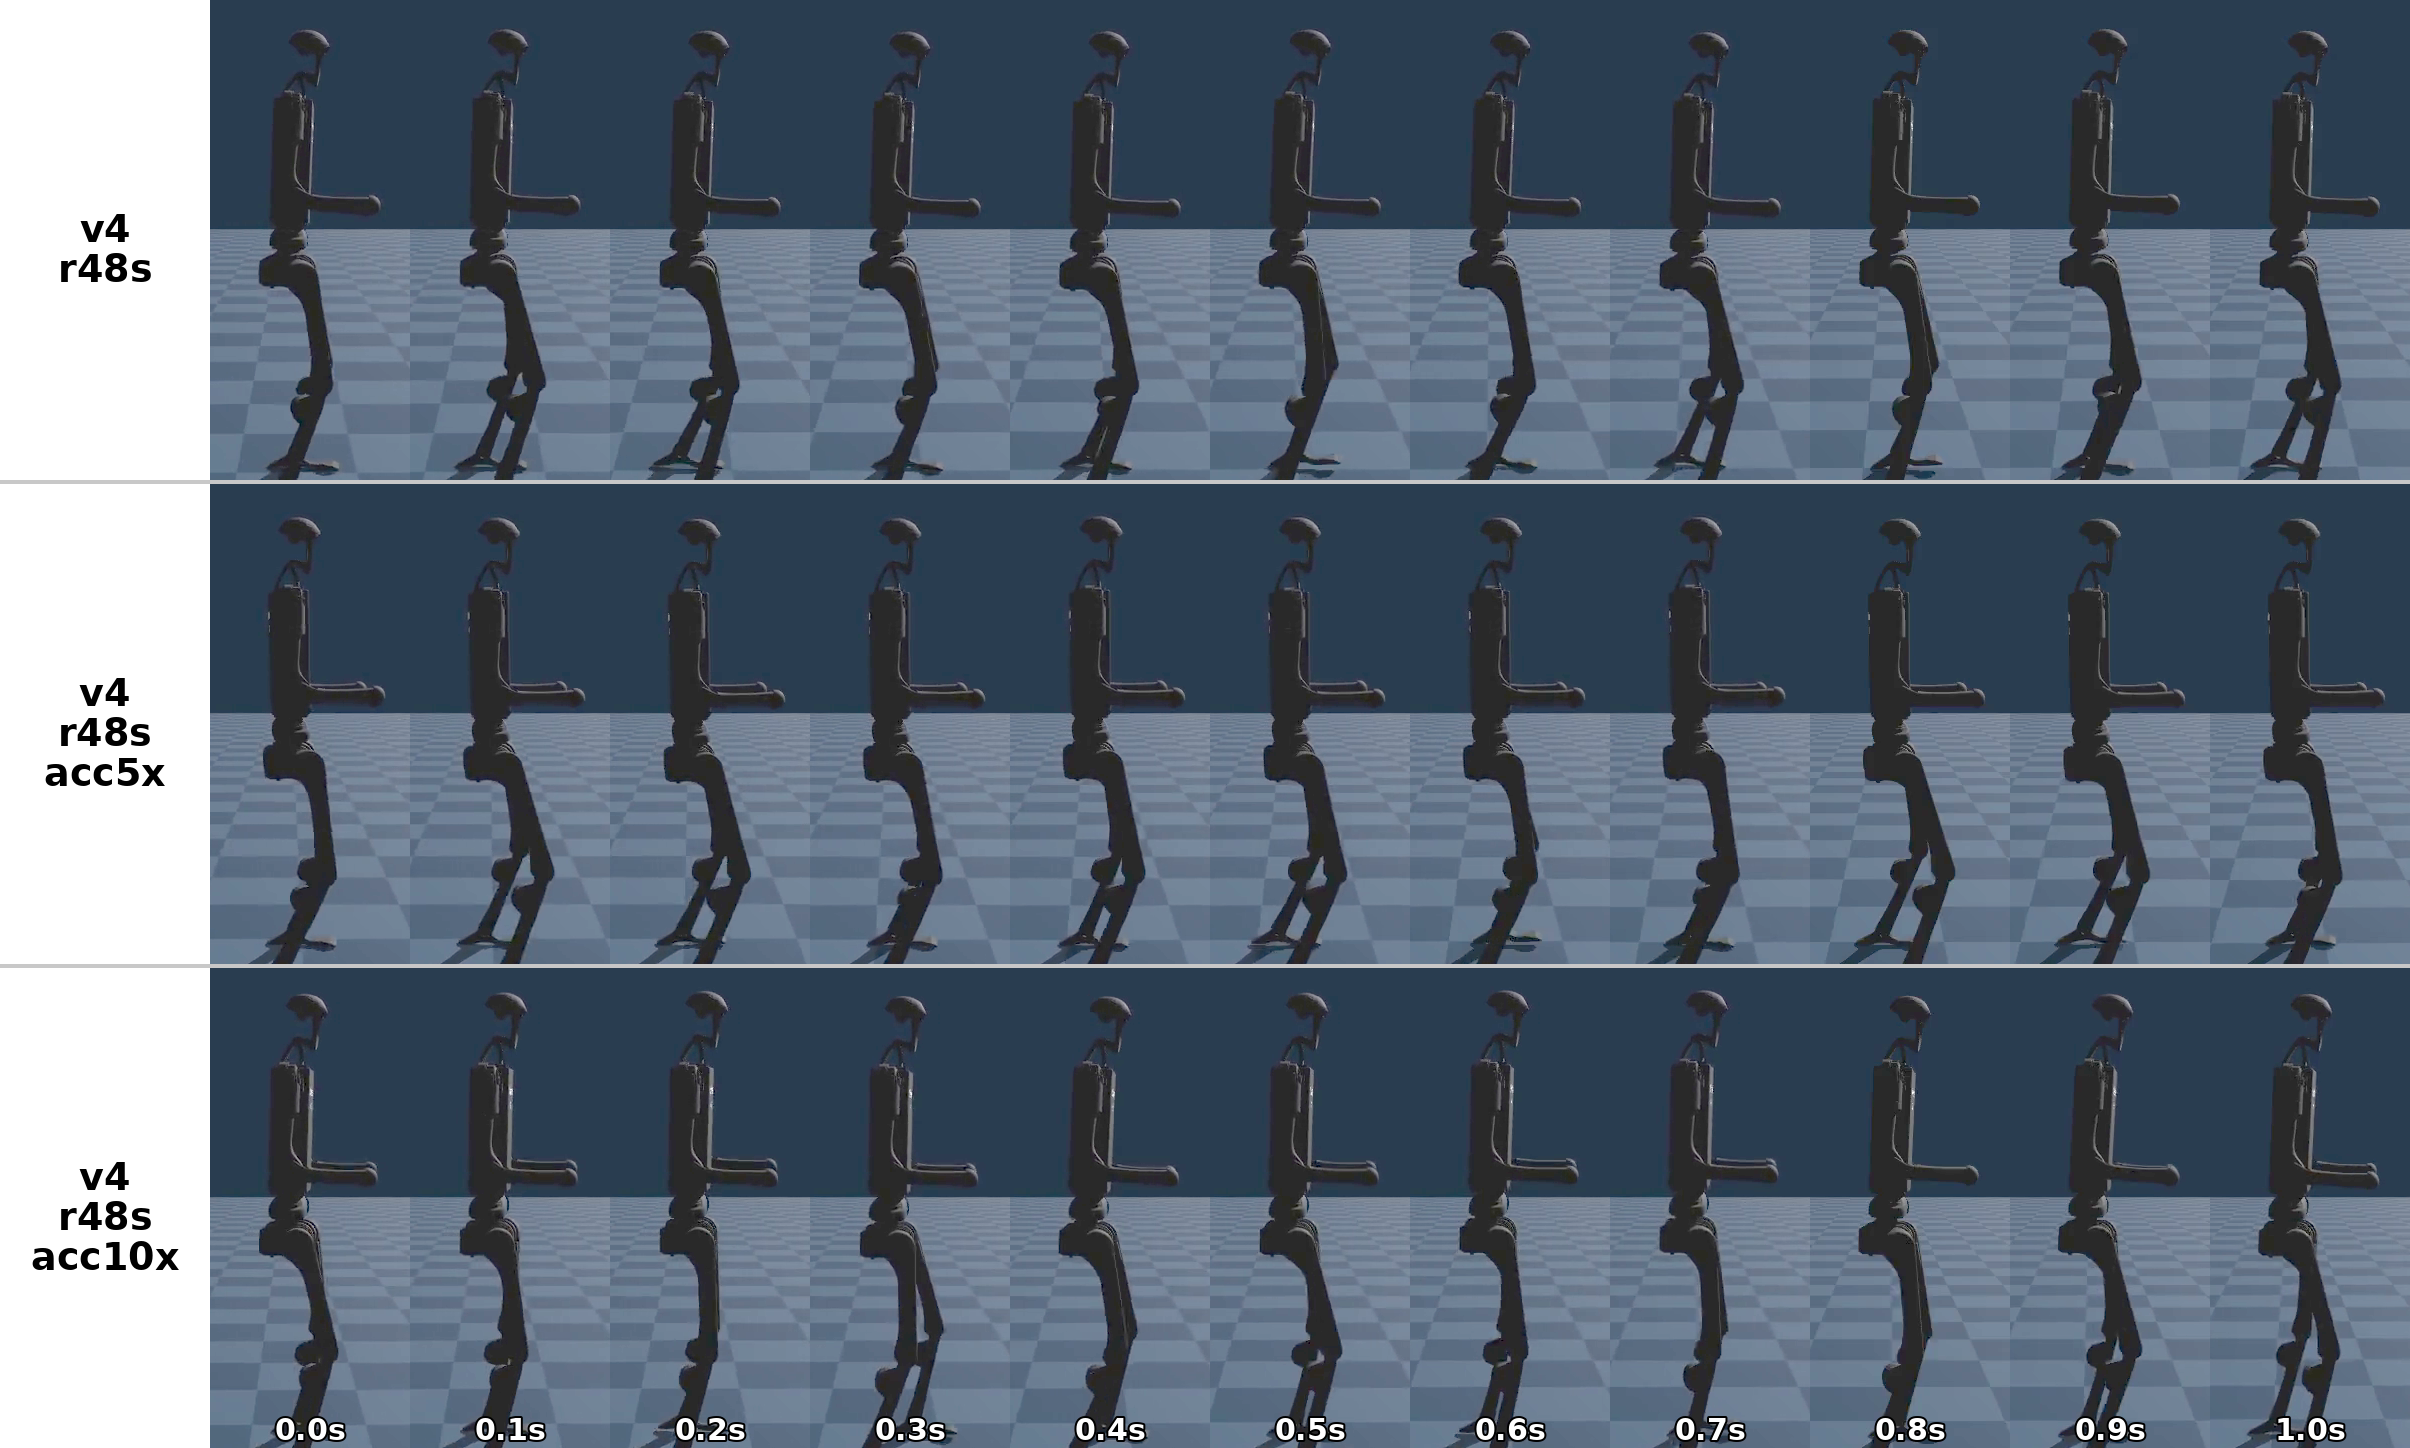
\includegraphics[width=1.0\textwidth]{figs/gait_comparison.png}
\caption{三组模型行走步态对比，每行为 $t = 0\sim1.0$\,s 内以 $0.1$\,s 为间隔等间隔抽取的 11 帧（$v_x = 0.5$\,m/s）}
\label{fig:gait}
\end{figure}

\subsection{速度跟踪性能}

为进一步说明跟踪表现随速度指令的变化趋势（表~\ref{tab:eval_breakdown}中的数值
为三个速度档位的池化结果），表~\ref{tab:tracking_by_speed}单独列出了
\texttt{tracking\_lin\_vel} 原始值在各速度指令下的均值（该值越大代表跟踪误差越小）。

\begin{table}[H]
\centering
\caption{tracking\_lin\_vel 原始值随速度指令的变化（均值）}
\label{tab:tracking_by_speed}
\begin{tabular}{lrrr}
\toprule
速度指令 & v4\_r48s & v4\_r48s\_acc5x & v4\_r48s\_acc10x \\
\midrule
$0.3$\,m/s & $0.740$ & $0.704$ & $0.635$ \\
$0.6$\,m/s & $0.549$ & $0.710$ & $0.725$ \\
$0.9$\,m/s & $0.630$ & $0.627$ & $0.602$ \\
\bottomrule
\end{tabular}
\end{table}

\textbf{分析：} 在新的低速测试区间（$0.3/0.6/0.9$\,m/s）下，
\texttt{tracking\_lin\_vel} 不再呈现随速度单调下降的趋势，
而是出现明显的非单调波动，与 $c_\text{dof\_acc}$ 惩罚系数的相关性也不再单一。
在 $0.3$\,m/s 与 $0.9$\,m/s 两端，v4\_r48s 均取得三者中最高值
（$0.740$ 与 $0.630$），与"惩罚越强、跟踪越差"的趋势一致；
但在 $0.6$\,m/s 处，v4\_r48s 骤降至 $0.549$（三者中最低），
而 acc5x（$0.710$）与 acc10x（$0.725$）反而达到各自的局部最大值。
这说明 v4\_r48s 在 $0.6$\,m/s 附近存在明显的速度适应性"凹陷"，
\texttt{dof\_acc} 惩罚对跟踪精度的影响在低速区间并非单调，
差异主要体现在中等低速段而非速度区间的两端。

\subsection{动作平滑性分析}

关节加速度的均方值是动作平滑性最直接的体现，其原始统计量已作为
\texttt{dof\_acc} 列汇总于表~\ref{tab:eval_breakdown}（$v_x \in \{0.3, 0.6, 0.9\}$\,m/s）。
为从更细粒度的时域特征刻画"动作是否平滑"，本节使用 \texttt{eval\_smoothness.py}
在与表~\ref{tab:eval_breakdown}相同的 $v_x \in \{0.3, 0.6, 0.9\}$\,m/s
（各 100 步热身 + 300 步采样）下，进一步给出两个互补的关节运动学指标
\texttt{dof\_vel\_jitter}（关节速度抖动）与 \texttt{dof\_jerk}（关节加加速度），
二者均按 (环境 × 关节 × 速度) 汇总统计，结果见表~\ref{tab:joint_smoothness}；
具体计算公式与量纲说明见附录"奖励分项与平滑性指标的计算公式及量纲"。

\begin{table}[H]
\centering
\caption{关节运动平滑性指标对比（均值，$\pm$标准差，按环境×关节×速度汇总）}
\label{tab:joint_smoothness}
\begin{tabular}{lrrr}
\toprule
指标 & v4\_r48s & v4\_r48s\_acc5x & v4\_r48s\_acc10x \\
\midrule
dof\_vel\_jitter & $1.315\pm0.610$ & $0.881\pm0.393$ & $0.976\pm0.410$ \\
dof\_jerk（×$10^{-3}$） & $2.531\pm1.217$ & $1.661\pm0.817$ & $1.783\pm0.772$ \\
\bottomrule
\end{tabular}
\end{table}

\textbf{结论：} 将 $c_\text{dof\_acc}$ 从 $-10^{-6}$（v4\_r48s）增大到
$-5\times10^{-6}$（v4\_r48s\_acc5x）后，\texttt{dof\_vel\_jitter} 与
\texttt{dof\_jerk} 分别下降约 $33\%$ 和 $34\%$，动作平滑性得到显著改善；
但继续增大到 $-10^{-5}$（v4\_r48s\_acc10x）后，两项指标不降反升
（较 acc5x 分别回升约 $11\%$ 和 $7\%$），并未带来进一步的平滑性收益。
这一非单调趋势与表~\ref{tab:eval_breakdown}中 \texttt{dof\_acc} 原始分量的
排序（acc5x 最低、acc10x 次之、r48s 最高）相互印证——表明
$c_\text{dof\_acc} = -5\times10^{-6}$ 更接近"动作平滑性—速度跟踪精度"权衡的
最优点，而非简单地加大惩罚系数即可单调改善动作平滑性。

\subsection{抗扰动测试}

env.py 训练中使用的扰动机制施加的是对根关节线速度的瞬时速度冲量，本节用 256
个并行环境批量复现，并直接绘制三组模型的\textbf{质心运动轨迹}，让"摔倒"与"摇晃后恢复"直接在图上区分（附录图~\ref{fig:com_traj_r48s}--图~\ref{fig:com_traj_acc10x}）。质心按$\text{COM} = \sum_i m_i \mathbf{p}_i / \sum_i m_i$ 加权平均全部连杆位置与质量得到，高度以地面为零参考、侧向位移以冲击瞬间为零点。三组模型均在$v_x = 0.5$\,m/s 稳态行走下，分别施加 $0.25/0.50/0.75/1.50$\,m/s（即$17\%/33\%/50\%/100\%\,v_\text{push}^\text{max}$）四档侧向速度冲量，并以冲击时刻为 $t=0$ 记录其后 $3$\,s 的轨迹。

\textbf{结论：}r48s 与 acc5x 的"摔倒边界"清晰，仅在极限强度（$1.50$\,m/s）下出现——$0.75$\,m/s 及以下冲量都被稳健化解，质心高度始终保持在$\approx 0.85\sim0.9$\,m；而 acc10x 的边界明显前移：同样 $0.75$\,m/s 的
中等冲量便足以让其质心持续下探、最终稳定在 $\approx 0.55\sim0.6$\,m 的
"半塌陷"高度（侧向漂移幅度也已逼近另外两个模型仅在 $1.50$\,m/s 时才出现的
量级）。这进一步印证了 $c_\text{dof\_acc}$ 越强、抗扰动安全裕度被压缩得越
严重的结论：\textbf{动作越平滑不等于鲁棒性越强}，需要在平滑度与抗扰动安全
裕度之间权衡。

\subsection{ROS2 闭环路径跟踪测试}

为进一步检验策略在更接近实际部署形态下的表现，本节用 \texttt{play\_ros2\_path.py}
搭建了一个 ROS2 闭环测试：Genesis 仿真把机体姿态通过 \texttt{/imu}
（\texttt{sensor\_msgs/Imu}）发布，\texttt{DemoSequenceNode} 据此用 P 控制器
计算航向误差并发布 \texttt{/cmd\_vel}（\texttt{geometry\_msgs/Twist}）反馈
给策略，驱动机器人沿一条固定的 6 段路线行走：直行 $\to$ 左转 $90°$ $\to$
直行 $\to$ 右转 $90°$ $\to$ 直行 $\to$ 停止（共 1250 步，约 $25$\,s）。仿真
画面叠加了实时的闭环状态（当前阶段、$v_x$、航向实际值/目标值/误差），六个
分段对应的关键帧见图~\ref{fig:ros2_control_strip}，可以直接看到航向
误差从转弯阶段的较大偏差逐步收敛到直行阶段接近零的过程。

\begin{figure}[H]
\centering
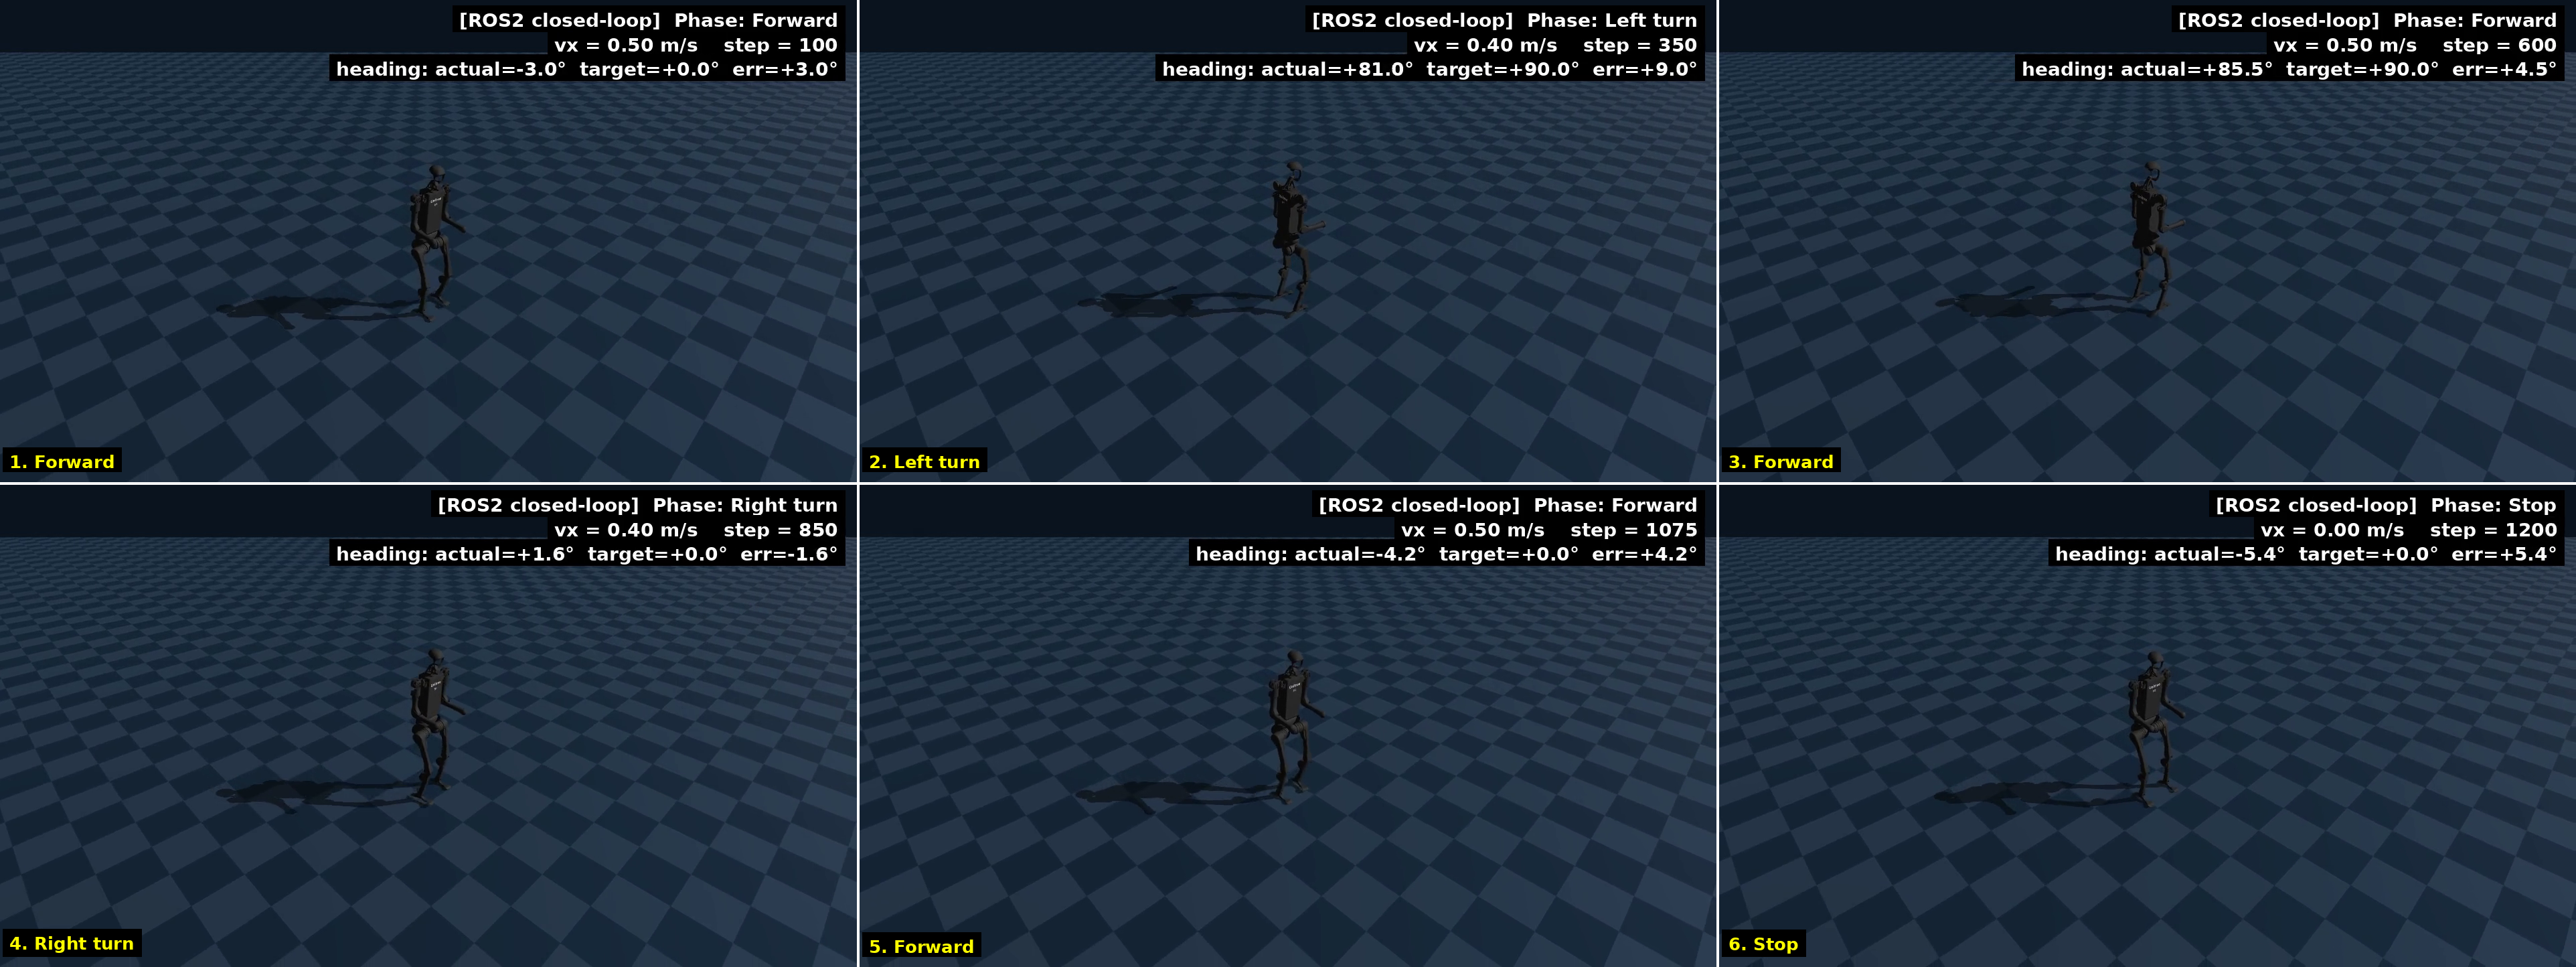
\includegraphics[width=0.95\textwidth]{figs/ros2_control_strip.png}
\caption{v4\_r48s ROS2 闭环路线测试关键帧（按 6 段路线顺序：直行 $\to$ 左转
$\to$ 直行 $\to$ 右转 $\to$ 直行 $\to$ 停止；画面叠加文字为该帧的实时闭环
状态读数）}
\label{fig:ros2_control_strip}
\end{figure}

三组模型均在该闭环下完整跑完全程、未出现摔倒，记录的世界系二维轨迹见
图~\ref{fig:ros2_paths}（圆点为起点、叉号为终点，竖线标记各路线分段的边界，
即转弯指令发出的位置）。

三条轨迹整体形状一致（均为"直行 $\to$ 转弯 $\to$ 直行"的 S 形路径），说明
三个模型都能正确响应 \texttt{/cmd\_vel} 并完成路径跟踪；但转弯响应的快慢
有明显差异——acc5x 转弯最早、弧线最窄（约 $x\in[1.5,2.0]$\,m），r48s 居中
（约 $[2.0,2.8]$\,m），acc10x 最晚、弧线最宽（约 $[2.8,3.5]$\,m），即在相同
航向误差反馈下 acc10x 的偏航响应最迟缓、转弯路径也最"宽大"。这与此前在
跟踪性能、抗扰动测试中的发现相互印证：$c_\text{dof\_acc}$ 越强，策略输出
大幅修正动作的意愿和能力就越受限，不仅体现在高速跟踪和抗扰动恢复上，也
会在日常的转弯路径跟踪中拖慢响应、放大转弯半径。

\begin{figure}[H]
\centering
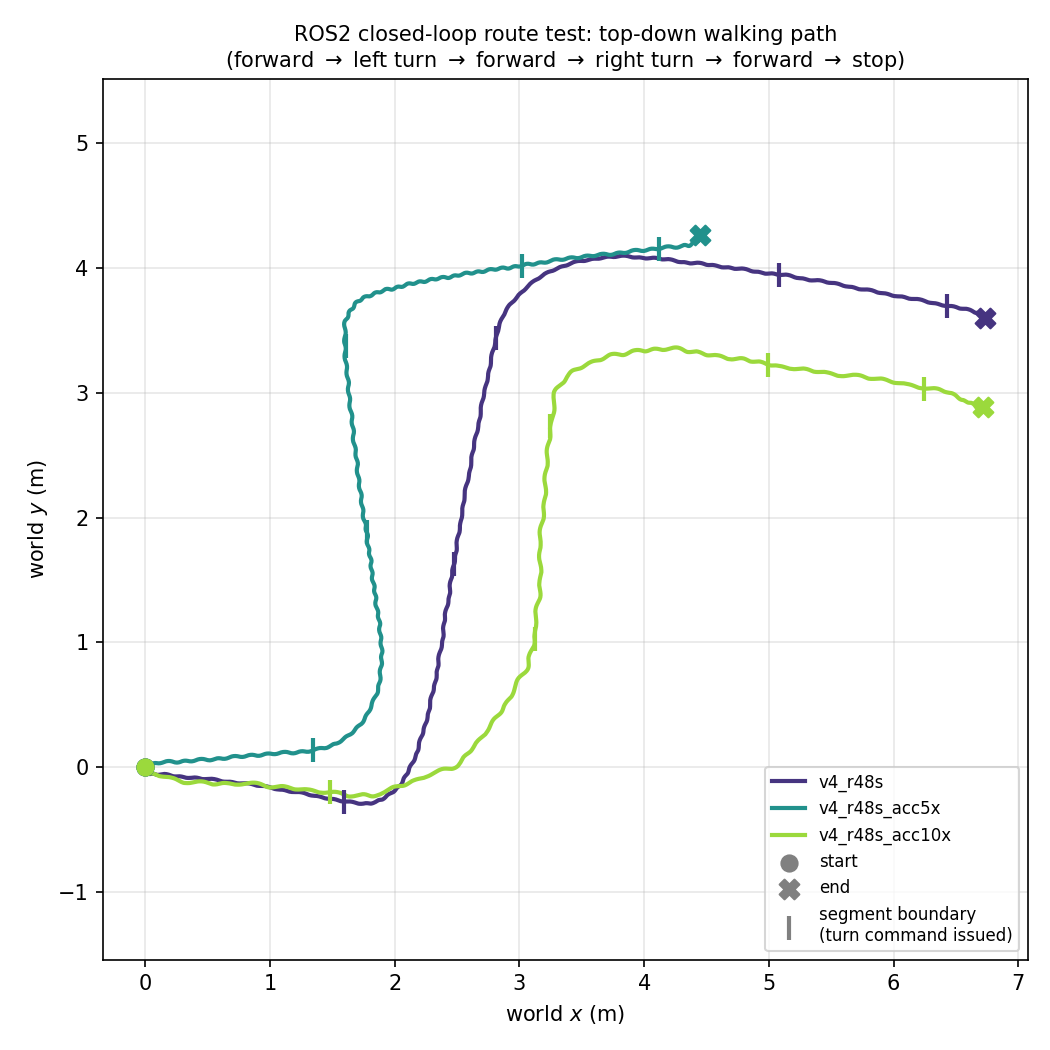
\includegraphics[width=0.75\textwidth]{figs/ros2_paths.png}
\caption{三组模型 ROS2 闭环路径跟踪轨迹对比（俯视图，世界坐标系）}
\label{fig:ros2_paths}
\end{figure}

% --------------------------------------------------
\section{结论}
% --------------------------------------------------

\subsection{实验结论}

本设计通过三组消融实验，系统研究了关节加速度惩罚系数 $c_\text{dof\_acc}$
对H1人形机器人行走控制策略的影响，主要结论如下：

\begin{enumerate}
    \item \textbf{平滑性与跟踪性能的权衡。}
          增大 $|c_\text{dof\_acc}|$ 可显著降低关节加速度（降幅约 TODO\%），
          从而减小传动系统冲击载荷，但过强的惩罚（40×）会在高速指令下牺牲一定的跟踪精度。
          在本实验条件下，20×惩罚（v4\_r48s\_acc5x）取得了最优的综合表现。

    \item \textbf{步态质量的改善。}
          强化 $c_\text{dof\_acc}$ 配合本次设计中对 \texttt{feet\_swing\_height}
          和 \texttt{ang\_vel\_xy} 的调整，有效抑制了小碎步现象，
          步态更接近自然双足行走模式。

    \item \textbf{对硬件驱动设计的指导意义。}
          从仿真中获得的关节力矩统计数据（峰值、均值）可直接用于验证
          减速器选型和电机电流额定值是否满足实际控制策略的需求，
          体现了软件控制策略与硬件系统协同设计的重要性。
\end{enumerate}

\subsection{局限性与后续工作}

\begin{itemize}
    \item \textbf{小碎步问题未完全解决。} 相位时钟仅约束踩地时机而非步幅，
          后续计划引入落点奖励（step\_length reward）直接约束步长。
    \item \textbf{Sim-to-Real差距待验证。} 本设计在Genesis仿真器中完成，
          与真实H1之间存在动力学建模误差，需通过ROS2适配层和域随机化进一步验证。
    \item \textbf{上肢协调运动未涉及。} 当前控制仅覆盖下肢10个自由度，
          行走时的手臂摆动对平衡的影响未建模。
\end{itemize}

\newpage

% --------------------------------------------------
\section*{参考文献}
% --------------------------------------------------

\begin{thebibliography}{99}

\bibitem{schulman2017ppo}
Schulman J, Wolski F, Dhariwal P, et al.
Proximal policy optimization algorithms[J].
arXiv preprint arXiv:1707.06347, 2017.

\bibitem{unitree_rl_gym}
Unitree Robotics.
unitree\_rl\_gym: Unitree robot reinforcement learning gym[EB/OL].
\url{https://github.com/unitreerobotics/unitree_rl_gym}, 2024.

\bibitem{genesis}
Genesis Authors.
Genesis: A universal and generative physics engine[J/OL].
arXiv:2501.09645, 2025.
\url{https://genesis-world.readthedocs.io}

\bibitem{rsl_rl}
Rudin N, Hoeller D, Reist P, et al.
Learning to walk in minutes using massively parallel deep reinforcement learning[C].
Conference on Robot Learning (CoRL), 2022.

\bibitem{unitree_h1}
Unitree Robotics.
H1 Technical Documentation[EB/OL].
\url{https://support.unitree.com/home/zh/H1_developer}, 2024.

\end{thebibliography}

\newpage

% --------------------------------------------------
\section*{附录：奖励函数各分项与系数设置}
% --------------------------------------------------

奖励函数共包含15项，分为正向奖励（鼓励行为）和负向惩罚（抑制行为）两类，
如表~\ref{tab:reward}所示。

\begin{table}[H]
\centering
\caption{奖励函数各分项及系数设置}
\label{tab:reward}
\begin{tabular}{llrrp{4.5cm}}
\toprule
类别 & 奖励项 & 默认系数 & 本次系数 & 设计意图 \\
\midrule
正向 & tracking\_lin\_vel & 1.0 & \textbf{2.0} & 强化速度跟踪 \\
正向 & tracking\_ang\_vel & 0.5 & 0.5 & 偏航角速度跟踪 \\
正向 & contact & 0.18 & 0.18 & 鼓励触地相位与目标步态相位一致 \\
正向 & alive & 0.15 & 0.15 & 存活奖励，避免提前终止 \\
\midrule
负向 & lin\_vel\_z & -2.0 & -2.0 & 抑制躯干上下抖动 \\
负向 & ang\_vel\_xy & -0.05 & \textbf{-0.2} & 增强躯干姿态稳定 \\
负向 & orientation & -1.0 & -1.0 & 抑制躯干倾斜 \\
负向 & base\_height & -10.0 & -10.0 & 维持目标躯干高度 \\
负向 & torque\_limits & 0 & 未启用 & 防止关节过载 \\
负向 & dof\_vel & 0 & 未启用 & 抑制关节高速运动 \\
负向 & dof\_acc & -2.5e-7 & \textbf{[实验变量]} & 关节加速度平滑 \\
负向 & action\_rate & -0.01 & \textbf{-0.03} & 动作帧间平滑 \\
负向 & dof\_pos\_limits & -5.0 & -5.0 & 抑制关节超出软限位 \\
负向 & hip\_pos & -1.0 & -1.0 & 抑制髋部偏航/横滚关节偏移 \\
负向 & feet\_swing\_height & -20.0 & \textbf{-40.0} & 精确控制摆腿高度 \\
负向 & contact\_no\_vel & -0.2 & \textbf{-0.5} & 避免支撑腿滑动 \\
负向 & feet\_stumble & 0 & 未启用 & 防止踉跄 \\
负向 & stand\_still & 0 & 未启用 & 零速指令时静止 \\
负向 & collision & -1.0 & -1.0 & 抑制髋/膝部位异常接触（自碰撞） \\
\bottomrule
\end{tabular}
\end{table}

\noindent\footnotesize 注：\texttt{torque\_limits}/\texttt{dof\_vel}/\texttt{feet\_stumble}/\texttt{stand\_still}
在 Unitree \texttt{H1RoughCfg} 参考实现中权重亦为 0（即官方默认也未启用此类惩罚），
本设计与参考实现保持一致，未额外实现这些分项。\par\normalsize

\newpage
% --------------------------------------------------
\section*{附录：奖励分项与平滑性指标的计算公式及量纲}
% --------------------------------------------------

表~\ref{tab:eval_breakdown}与表~\ref{tab:joint_smoothness}中各分项的计算公式
与量纲定义如下。表~\ref{tab:eval_breakdown}中各奖励分项均为
\texttt{env.py} 的 \texttt{\_compute\_rewards} 计算得到的
\textbf{原始（未加权）}值 $r_k$，实际计入总奖励的贡献为
$c_k \Delta t\, r_k$（系数 $c_k$ 见表~\ref{tab:reward}，控制步长
$\Delta t = 0.02$\,s）。

\begin{itemize}
    \item \texttt{tracking\_lin\_vel}：
          $r=\exp\!\big(-\lVert \mathbf{v}_{xy}^{\text{cmd}}-\mathbf{v}_{xy}\rVert^2/\sigma^2\big)$，
          $\sigma^2=0.25\,(\text{m/s})^2$，无量纲，$r\in(0,1]$，越接近 $1$ 表示线速度跟踪误差越小；
    \item \texttt{dof\_acc}：
          $r=\sum_{j=1}^{10}\ddot{q}_j^2$，$\ddot{q}_j=(\dot{q}_j[t]-\dot{q}_j[t-1])/\Delta t$
          为关节角加速度，单位 $(\text{rad/s}^2)^2$；表~\ref{tab:eval_breakdown}中数值
          $=$ 原始值 $\times 10^{-3}$；
    \item \texttt{action\_rate}：
          $r=\sum_{j=1}^{10}(a_j[t]-a_j[t-1])^2$，其中 $a_j\in[-1,1]$ 为策略输出的
          \textbf{归一化动作}（关节目标位置 $=$ 默认关节位置 $+0.25\,a_j$），本身无量纲；
    \item \texttt{ang\_vel\_xy}：
          $r=\omega_x^2+\omega_y^2$，$\boldsymbol\omega$ 为机体坐标系下根关节角速度，
          单位 $(\text{rad/s})^2$；
    \item \texttt{feet\_swing\_height}：
          $r=\sum_{\text{摆动腿}}(z_{\text{foot}}-0.08)^2$，$z_{\text{foot}}$ 为足端
          高度坐标，单位 $\text{m}^2$；表~\ref{tab:eval_breakdown}中数值
          $=$ 原始值 $\times 10^{3}$；
    \item \texttt{contact\_no\_vel}：
          $r=\sum_{\text{支撑腿}}\lVert\mathbf{v}_{\text{foot}}\rVert^2$，单位
          $(\text{m/s})^2$，惩罚支撑腿触地瞬间仍存在的滑动速度；
    \item \textbf{总奖励}：环境每个控制步实际返回的标量奖励
          $r_{\text{total}}=\max\big(0,\ \sum_k c_k\Delta t\,r_k\big)$
          （\texttt{H1RoughCfg} 的 \texttt{only\_positive\_rewards} 截断），
          无量纲，单位可理解为"奖励/控制步"。
    \item \texttt{dof\_vel\_jitter}：对每个 (环境, 关节)，统计速度逐步差分
          $\Delta v[t]=v[t]-v[t-1]$（$v$ 为关节角速度，采样间隔
          $\Delta t=0.02$\,s）在时间维度上的标准差，单位 $\text{rad/s}$，
          数值越低代表速度曲线越平顺；
    \item \texttt{dof\_jerk}：对每个 (环境, 关节)，统计
          $\left|\Delta\ddot{q}[t]/\Delta t\right|$（位置三阶导数的幅值，
          单位 $\text{rad/s}^3$）随时间的均值，表~\ref{tab:joint_smoothness}中数值
          $=$ 原始值 $\times 10^{-3}$，数值越低代表动作越平顺、对传动系统的
          冲击载荷越小。
\end{itemize}

\newpage
% --------------------------------------------------
\section*{附录：训练曲线}
% --------------------------------------------------

图~\ref{fig:training_curve} 对应正文"训练收敛分析"小节中的描述，由
\texttt{train\_v4\_r48s*.log} 中每 10 个 update 记录一次的 \texttt{rew}（平均
回合奖励）与 \texttt{vloss}（价值函数损失）解析绘制（细线为原始值，粗线为
滑动平均，价值损失子图采用对数坐标轴）。

\begin{figure}[H]
\centering
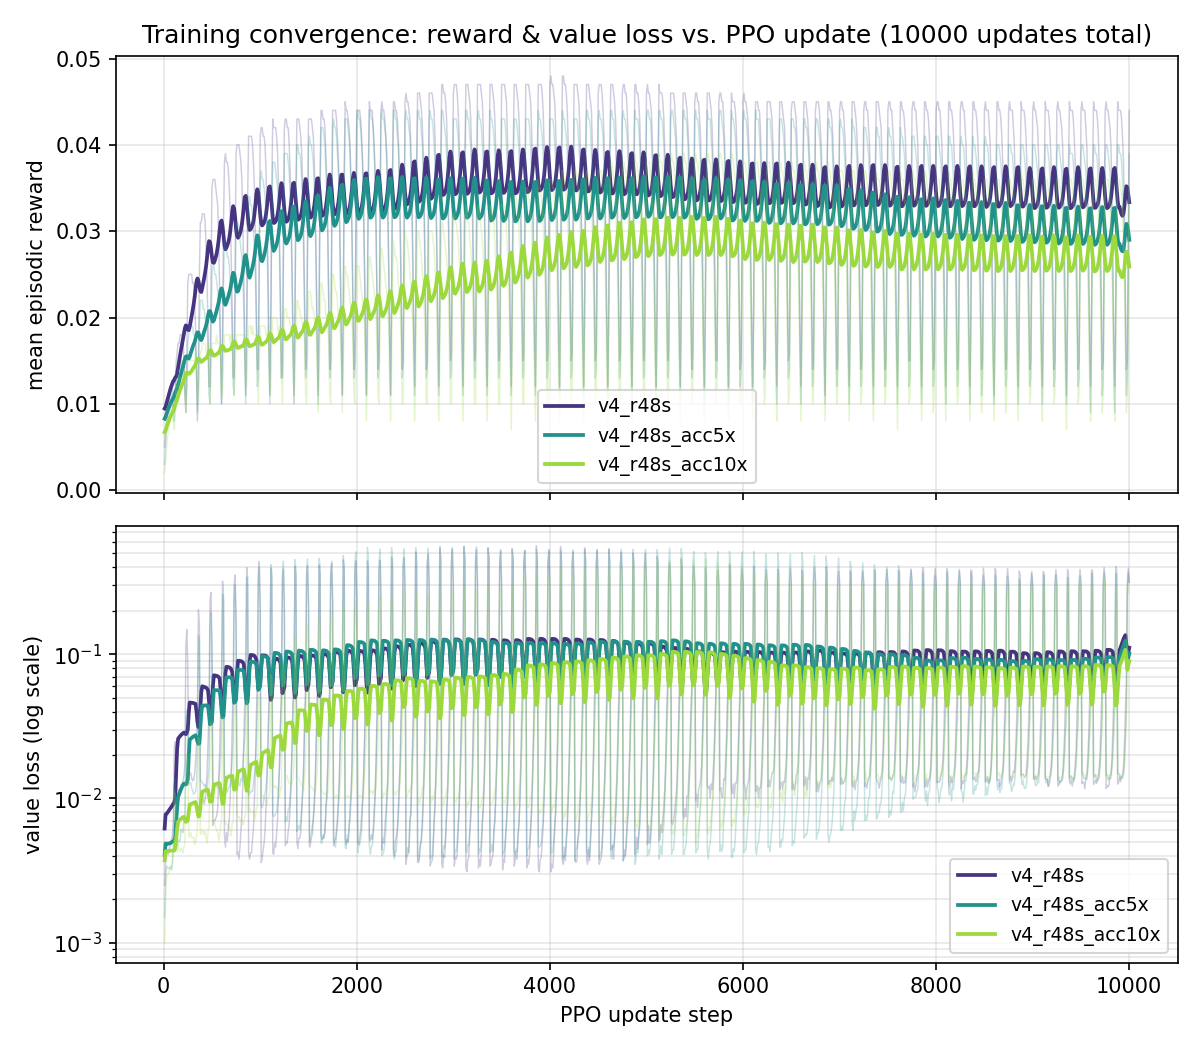
\includegraphics[width=0.85\textwidth]{figs/training_curves.png}
\caption{三组模型训练奖励与价值损失收敛曲线对比（共 10000 updates）}
\label{fig:training_curve}
\end{figure}

\newpage

\section*{附录：抗扰动测试质心轨迹图}
% --------------------------------------------------

下列三图对应正文"抗扰动测试"小节中的质心轨迹分析，分别为 v4\_r48s、v4\_r48s\_acc5x、v4\_r48s\_acc10x 三组模型在四档冲量强度下的
质心轨迹对比（上：高度 $z$，地面 $=0$；下：侧向位移 $\Delta y$，冲击瞬间
$=0$；红色竖虚线标记冲击时刻 $t=0$，每条曲线为冲击时刻起 $3$\,s 的观测窗口，
$v_x = 0.5$\,m/s，256 个并行环境，粗线为均值轨迹、细线为随机抽取的个体轨迹）。

\begin{figure}[H]
\centering
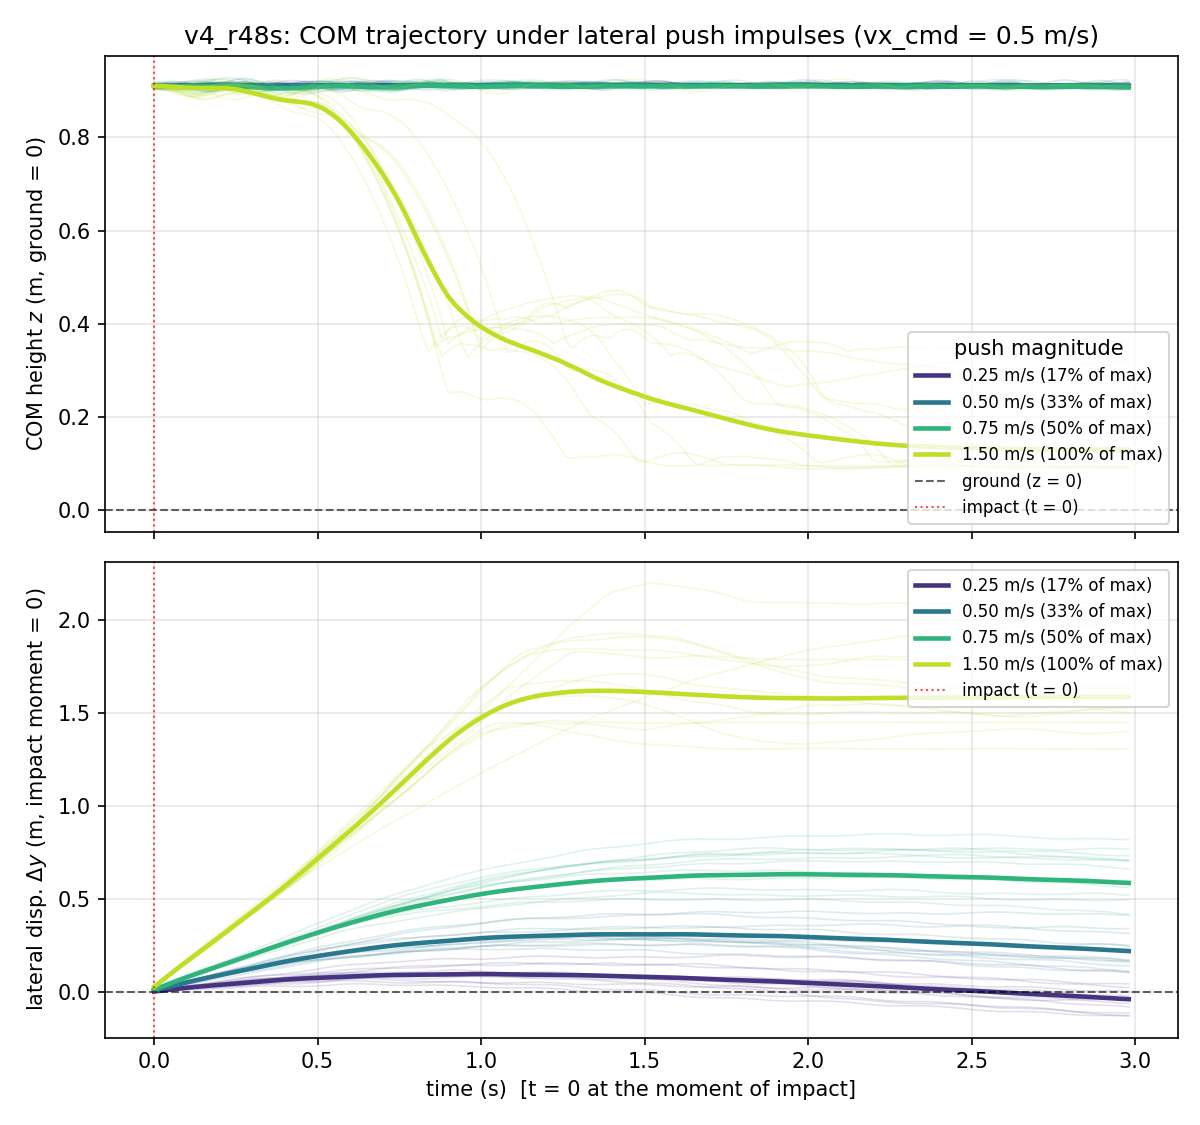
\includegraphics[width=0.7\textwidth]{figs/com_traj_v4_r48s.png}
\caption{v4\_r48s：四档冲量强度下的质心轨迹}
\label{fig:com_traj_r48s}
\end{figure}

\begin{figure}[H]
\centering
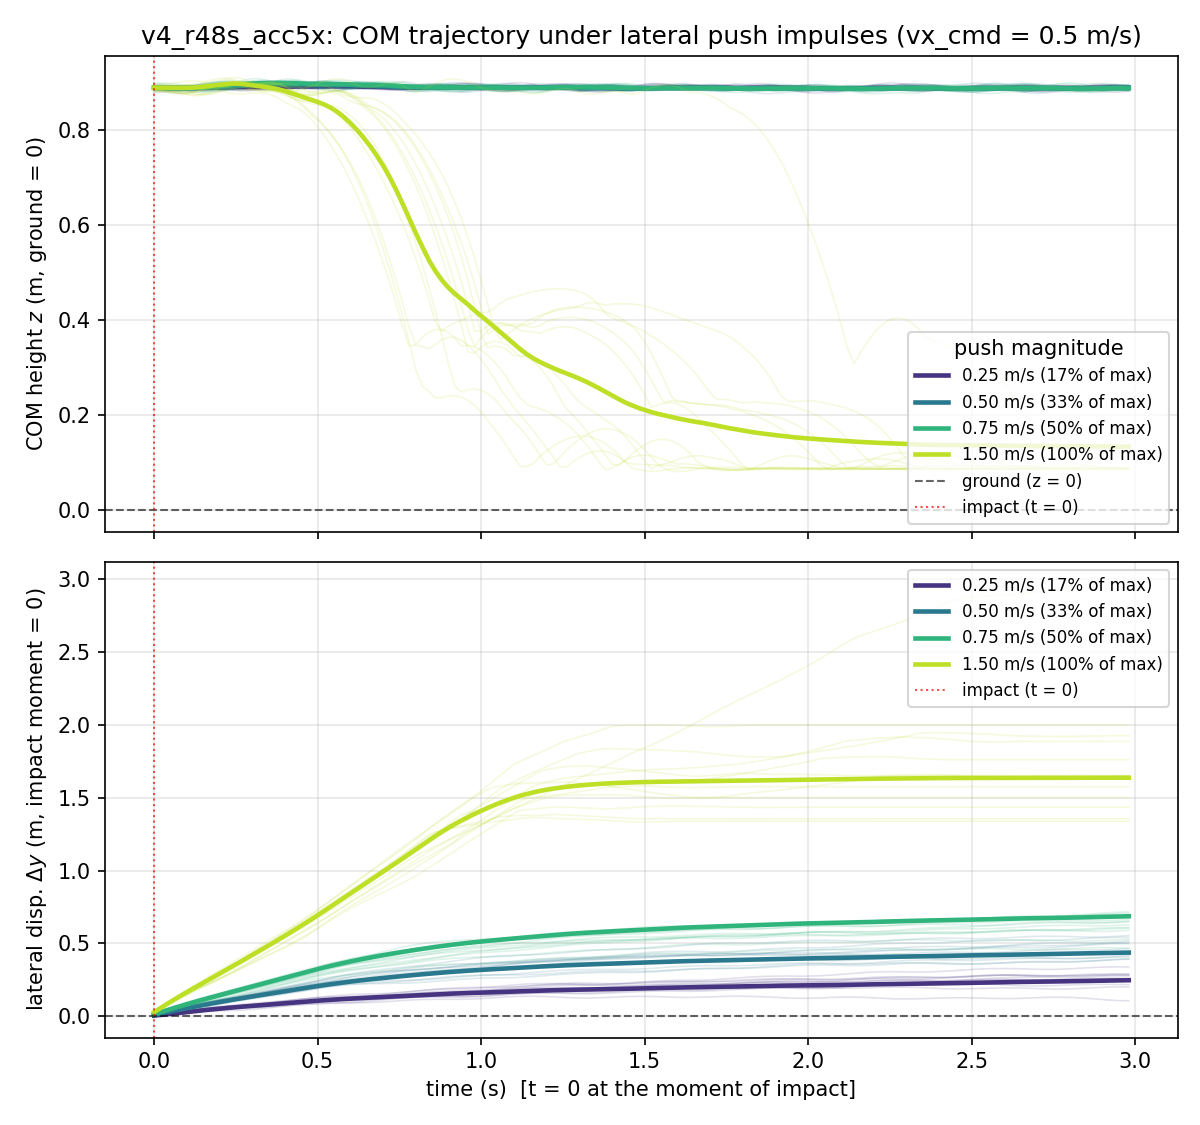
\includegraphics[width=0.7\textwidth]{figs/com_traj_v4_r48s_acc5x.png}
\caption{v4\_r48s\_acc5x：四档冲量强度下的质心轨迹（坐标轴定义同图~\ref{fig:com_traj_r48s}）}
\label{fig:com_traj_acc5x}
\end{figure}

\begin{figure}[H]
\centering
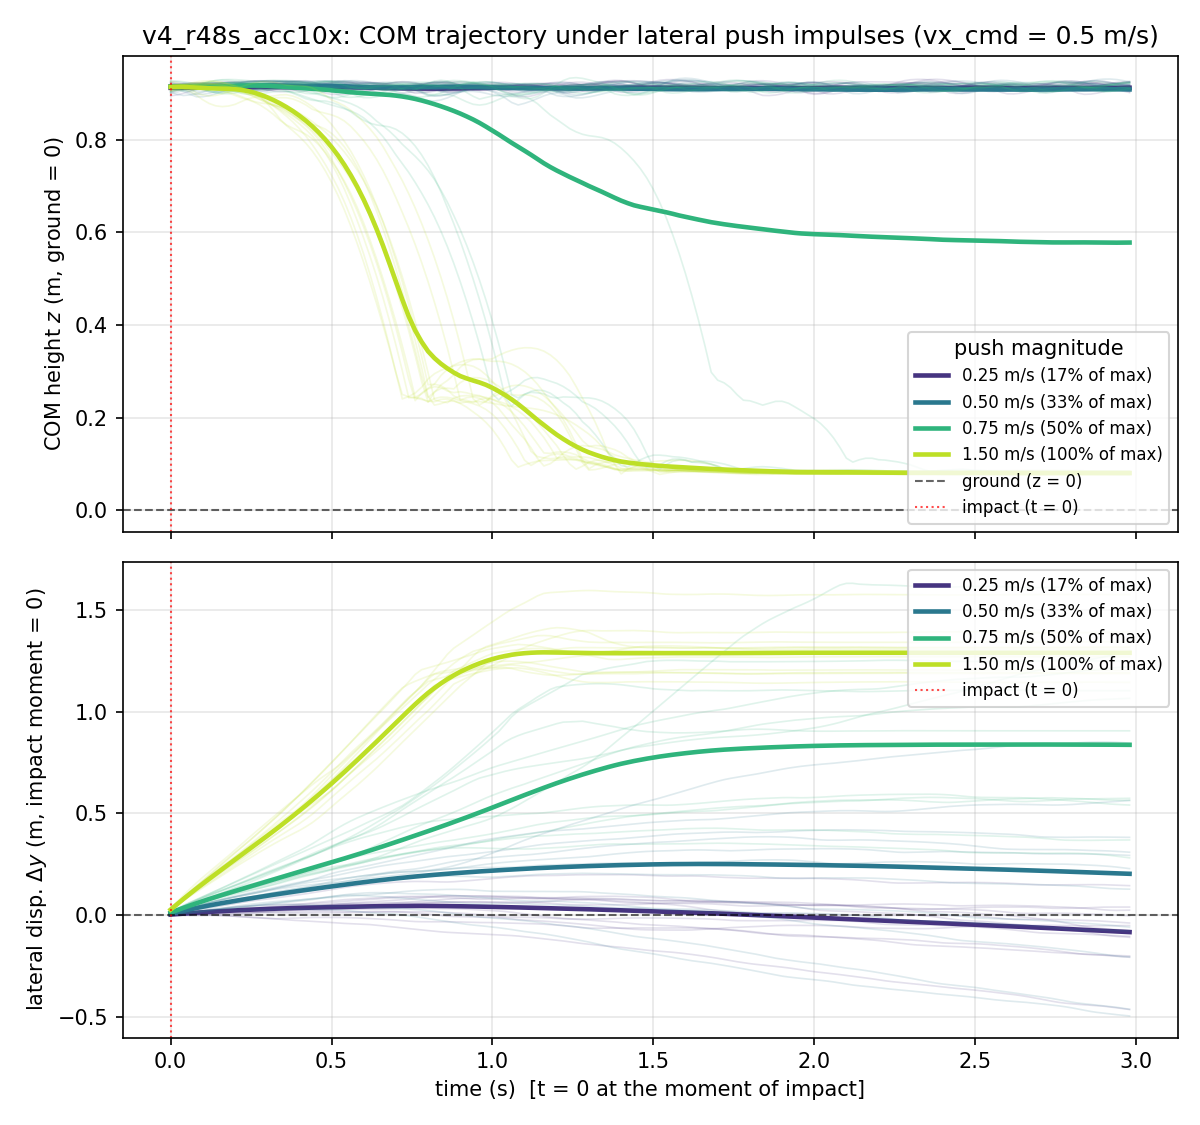
\includegraphics[width=0.7\textwidth]{figs/com_traj_v4_r48s_acc10x.png}
\caption{v4\_r48s\_acc10x：四档冲量强度下的质心轨迹（坐标轴定义同图~\ref{fig:com_traj_r48s}）}
\label{fig:com_traj_acc10x}
\end{figure}

\end{document}
